\documentclass[10pt]{article}
\usepackage[utf8]{inputenc}
\usepackage[english]{babel}
\usepackage[left=2cm, right=2cm, top=2cm, bottom=2cm]{geometry}
\usepackage{amsmath, wrapfig, pgfplots}

\pgfplotsset{compat=1.9}

\begin{document}

\title{Cascaded Approximation of Gaussian Blur}
\author{Vabishchevich Nikolay}
\date{May 14, 2015}
\maketitle


\section{Basic definitions}

\begin{wrapfigure}{r}{0pt}
    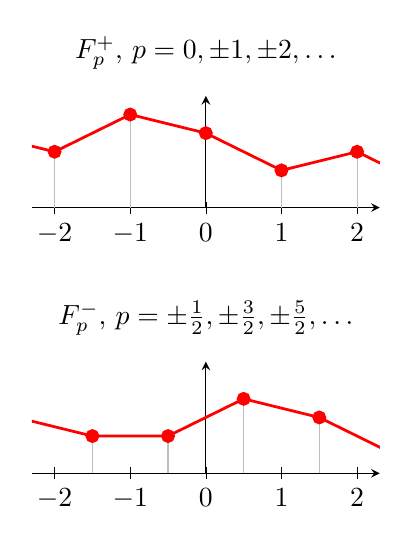
\begin{tikzpicture}
        \begin{axis} [ width = 6cm, height = 3cm, name = plot,
                title = {$F^+_p$, $p = 0, \pm1, \pm2, \ldots$},
                xmin = -2.3, xmax = 2.3, axis x line = bottom,
                xtick = {-2, ..., 2}, x tick style = { color = black },
                ymin = 0, ymax = 6, axis y line = middle, ytick = \empty ]
            \addplot [ sharp plot, mark = *, line width = 1pt, red ] coordinates
                { (-3, 4) (-2, 3) (-1, 5) (0, 4) (1, 2) (2, 3) (3, 1) };
            \addplot [ ycomb, lightgray ] coordinates
                { (-2, 3) (-1, 5) (1, 2) (2, 3) };
        \end{axis}
        \begin{axis} [ width = 6cm, height = 3cm,
                at = { (plot.below south) }, anchor = above north, yshift = -0.5cm,
                title = {$F^-_p$, $p = \pm\frac12, \pm\frac32, \pm\frac52, \ldots$},
                xmin = -2.3, xmax = 2.3, axis x line = bottom, xtick = {-2, ..., 2}, x tick style = { color = black },
                ymin = 0, ymax = 6, axis y line = middle, ytick = \empty ]
            \addplot [ sharp plot, mark = *, line width = 1pt, red ] coordinates
                { (-2.5, 3) (-1.5, 2) (-0.5, 2) (0.5, 4) (1.5, 3) (2.5, 1) };
            \addplot [ ycomb, lightgray ] coordinates
                { (-1.5, 2) (-0.5, 2) (0.5, 4) (1.5, 3) };
        \end{axis}
    \end{tikzpicture}
    \caption{Two types of grid placement.}
\end{wrapfigure}

In this article I'm using two different sets of grid point positions. The first one is grid point at
every integer, $F^+_k$ (I call it even and mark with ``$+$''). The second one is grid points positioned
halfway between adjacent integers, $F^-_{k+1/2}$ (I call it odd and mark with ``$-$'').
Correspondingly there are two types of convolution filters: even
\begin{equation}\label{conv+}
    R^\pm_p = \sum_{k\in Z} F^\pm_{p+k}K^+_k,
\end{equation}
and odd
\begin{equation}\label{conv-}
    R^\mp_p = \sum_{k\in Z} F^\pm_{p+k+\frac12}K^-_{k+\frac12},
\end{equation}
where $K^\pm_p$ is filter kernel. Even filter doesn't change source oddness but odd filter do (hence
the name). Therefore our target problem is to effectively calculate approximation of
\begin{equation}
    R^\pm_p = \sum_{k\in Z} F^\pm_{p+k}G_k,
\end{equation}
where $F^\pm_p$ is the source function and $G_k$ is even gaussian kernel,
\begin{equation}\label{gauss_n}
    G_k = \frac1{\sqrt{2\pi\sigma^2}}\exp\left\{-\frac{k^2}{2\sigma^2}\right\},
\end{equation}
especially for large standard deviation $\sigma$.

The main tool for such task is the Fourier transform. I'm using it in the following form:
\begin{align}
    F^+(\varphi) &= \sum_{k\in Z} F^+_k e^{ik\varphi},\\
    F^-(\varphi) &= \sum_{k\in Z} F^-_{k+\frac12} e^{i(k+\frac12)\varphi},
\end{align}
\begin{equation}
    F^\pm_p = \frac1{2\pi}\int_{-\pi}^\pi F^\pm(\varphi)e^{-ip\varphi}d\varphi.
\end{equation}
As usual, Fourier transform of real function satisfies
\begin{equation}
    F^\pm(-\varphi) = F^{\pm*}(\varphi).
\end{equation}
Also due to discreteness holds the following (another source of the even/odd name):
\begin{equation}
    F^\pm(\varphi+2\pi) = \pm F^\pm(\varphi).
\end{equation}
For symmetric (relative to 0) functions its Fourier amplitude is strictly real.

For convolutional filter with even kernel $K^+_p$ (\ref{conv+}) holds
\begin{equation}
    R^\pm(\varphi) = F^\pm(\varphi)K^{+*}(\varphi).
\end{equation}
In case of odd kernel $K^-_p$ (\ref{conv-}),
\begin{equation}
    R^\mp(\varphi) = F^\pm(\varphi)K^{-*}(\varphi).
\end{equation}
For symmetric filters it's possible to drop conjugation sign in these equations.

In the following I'll need transforms of basic binomial filters. That's well known sequence of
filters, kernels of which from the beginning of the sequence look like
\begin{align}
    \label{B1} B^1 &= [1, 1] / 2,\\
    \label{B2} B^2 &= [1, 2, 1] / 4,\\
    \label{B3} B^3 &= [1, 3, 3, 1] / 8,\\
    \label{B4} B^4 &= [1, 4, 6, 4, 1] / 16,\\
    \label{B5} B^5 &= [1, 5, 10, 10, 5, 1] / 32,\\
    \label{B6} B^6 &= [1, 6, 15, 20, 15, 6, 1] / 64,\\
                   &\cdots\nonumber
\end{align}
Filters from the sequence at even index is even and of odd index is odd. Also it's easy to see that
effect from high order filter $B^n$ is the same as from the first filter $B^1$ (or simply $B$) applied
$n$ times. Hence its Fourier transform is
\begin{equation}
    B^n(\varphi) = \cos^n\frac\varphi2.
\end{equation}

\pgfplotsset{spectrum/.style = {
    width = 6cm, height = 6cm, domain = -1:1, samples = 256,
    xtick = {-1, 0, 1}, xticklabels = {$-\pi$, $0$, $\pi$}, minor x tick num = 1,
    xmin = -1, xmax = 1, xminorgrids = true, xmajorgrids = true,
    ymin = 0, ymax = 1, yminorgrids = true, ymajorgrids = true,
}}
\begin{wrapfigure}{r}{0pt}
    \begin{tikzpicture}
        \begin{axis} [ spectrum, title = $G^+(\varphi)$ ]
            \addplot [ sharp plot, line width = 1pt, red ] gnuplot {
                exp(-8*(x*pi)^2)
            };
        \end{axis}
    \end{tikzpicture}
    \caption{Gaussian spectrum (\ref{gauss}) for $\sigma = 4$.}
\end{wrapfigure}

Going back to our gaussian filter (\ref{gauss_n}), its Fourier transform is another gaussian function
\begin{equation}\label{gauss}
    G^+(\varphi) \approx \exp\left\{-\frac{\sigma^2\varphi^2}2\right\}.
\end{equation}
That function has two different regions. The first is almost zero at high frequency and the second
is bell-like shape at low frequency. Correspondingly the task of approximation can be divided into
two subtasks described in the following sections.


\section{Zeroing high frequency}

The only way to avoid large filter kernels in approximation of gaussian blur with large radius is to
somehow reduce resolution before filtering. That can be done through successive steps of shrinking by
factor of two, then applying main filter and then expanding twofold the same number of steps.
Central main filter will be examined in the next section and this section concentrates on scaling.

The basic operation for such task is dropping every second point from grid. For even function
$F^+_k$ there are two ways to do so. First is to keep only even points (I call it operator
$\hat S_+$)
\begin{equation}
    R^+_k = F^+_{2k}.
\end{equation}
Second is to keep odd (operator $\hat S_-$)
\begin{equation}
    R^-_{k+\frac12} = F^+_{2k+1}.
\end{equation}
Its Fourier transforms look like
\begin{equation}\label{S}
    R^\pm(\varphi) =
        \frac12 \left[F^+\left(\frac\varphi2\right) \pm F^+\left(\pi+\frac\varphi2\right)\right].
\end{equation}
Complementary operation for expanding is inserting zeroes between each neighbour pair of values.
Similarly there are two versions, even (operator $\hat S^\dagger_+$)
\begin{equation}
    R^+_n = \left\{
        \begin{array}{ll}
            F^+_k,& n = 2k;\\
            0,& n = 2k + 1.
        \end{array}
    \right.
\end{equation}
and odd (operator $\hat S^\dagger_-$ correspondingly)
\begin{equation}
    R^+_n = \left\{
        \begin{array}{ll}
            0,& n = 2k;\\
            F^-_{k+\frac12},& n = 2k + 1.
        \end{array}
    \right.
\end{equation}
Fourier transform of the result of that operation is quite direct
\begin{equation}
    R^+(\varphi) = F^\pm(2\varphi).
\end{equation}

\begin{figure}[t]
    \centering
    \begin{tikzpicture}
        \begin{axis} [ spectrum, name = plot1, title = $F^+$ ]
            \addplot [ sharp plot, line width = 1pt, domain = -1:-0.5, blue] gnuplot {
                0.8 * exp(-(x*pi)^2) + 0.4 * exp(-8*((abs(x)-1)*pi)^2)
            };
            \addplot [ sharp plot, line width = 1pt, domain = -0.5:0.5, green] gnuplot {
                0.8 * exp(-(x*pi)^2) + 0.4 * exp(-8*((abs(x)-1)*pi)^2)
            };
            \addplot [ sharp plot, line width = 1pt, domain = 0.5:1, blue] gnuplot {
                0.8 * exp(-(x*pi)^2) + 0.4 * exp(-8*((abs(x)-1)*pi)^2)
            };
        \end{axis}
    \end{tikzpicture}
    \begin{tikzpicture}
        \begin{axis} [ spectrum, name = plot2, title = $\hat S_+F^+$,
                at = { (plot1.right of east) }, anchor = left of west, xshift = 0.5cm ]
            \addplot [ sharp plot, line width = 1pt, green ] gnuplot {
                0.4 * exp(-(x*pi/2)^2)
            };
            \addplot [ sharp plot, line width = 1pt, blue ] gnuplot {
                0.4 * exp(-((abs(x/2)-1)*pi)^2) + 0.2 * exp(-8*(x*pi/2)^2)
            };
            \addplot [ sharp plot, line width = 1pt, red ] gnuplot {
                0.4 * exp(-(x*pi/2)^2) +
                0.4 * exp(-((abs(x/2)-1)*pi)^2) + 0.2 * exp(-8*(x*pi/2)^2)
            };
        \end{axis}
    \end{tikzpicture}
    \begin{tikzpicture}
        \begin{axis} [ spectrum, name = plot3, title = $\hat S^\dagger_+\hat S_+F^+$,
                at = { (plot2.right of east) }, anchor = left of west, xshift = 0.5cm ]
            \addplot [ sharp plot, line width = 1pt, red ] gnuplot {
                0.4 * exp(-(x*pi)^2) + 0.2 * exp(-8*((abs(x)-1)*pi)^2) +
                0.4 * exp(-((abs(x)-1)*pi)^2) + 0.2 * exp(-8*(x*pi)^2)
            };
        \end{axis}
    \end{tikzpicture}
    \caption{Spectrum of the source function $F^+(\varphi)$ after successive application of basic
        shrink $\hat S_+$ and expand $\hat S^\dagger_+$ operators.}
\end{figure}

Basic shrink/expand operations is not much useful as is due to several problems. Shrink operator
$\hat S_\pm$ isn't conservative ($R(\varphi)\neq F(\varphi)$) and high-frequency part contaminate
low-frequency. Expand operator $\hat S^\dagger_\pm$ duplicates low-frequency part into
high-frequency instead of zeroing it. To solve these problems I apply additional convolutional
filters before shrinking and after expanding. More particularly, the full shrink operator is
\begin{equation}\label{P}
    \hat P = 2\hat S\hat K_{\text{in}},
\end{equation}
where $2$ denotes multiplication by $2$ to get rid of $\frac12$ factor from (\ref{S}). The filter
kernel $K_{\text{in}}(\varphi)$ should be exactly zero at $\varphi = \pm\pi$ for conservation and be
quite small in all high half of the spectrum. Similarly, the full expand operator is
\begin{equation}\label{Q}
    \hat Q = \hat K_{\text{out}}\hat S^\dagger,
\end{equation}
where the filter kernel $K_{\text{out}}(\varphi)$ should be small at high-frequency.

Consider the following process: apply the shrink operator $\hat P$, then some convolutional filter
$\hat T$, than expand operator $\hat Q$. Fourier transform of the result can be easily calculated through
\begin{align}
    (\hat K_{\text{in}}F)(\varphi) &= K_{\text{in}}(\varphi)F(\varphi),\\
    (\hat PF)(\varphi) &=
        K_{\text{in}}\left(\frac\varphi2\right)F\left(\frac\varphi2\right) \pm
        K_{\text{in}}\left(\pi+\frac\varphi2\right)F\left(\pi+\frac\varphi2\right),\\
    (\hat T\hat PF)(\varphi) &= \left[
        K_{\text{in}}\left(\frac\varphi2\right)F\left(\frac\varphi2\right) \pm
        K_{\text{in}}\left(\pi+\frac\varphi2\right)F\left(\pi+\frac\varphi2\right)
        \right]T(\varphi),\\
    (\hat S^\dagger\hat T\hat PF)(\varphi) &= \left[K_{\text{in}}(\varphi)F(\varphi) \pm
        K_{\text{in}}(\pi+\varphi)F(\pi+\varphi)\right]T(2\varphi),\\
    R(\varphi) = (\hat Q\hat T\hat PF)(\varphi) &= \left[K_{\text{in}}(\varphi)F(\varphi) \pm
        K_{\text{in}}(\pi+\varphi)F(\pi+\varphi)\right]T(2\varphi)K_{\text{out}}(\varphi).
\end{align}
It's easy to see that there are two components in the result, good
\begin{equation}
    R_{\text{good}}(\varphi) =
        K_{\text{in}}(\varphi)T(2\varphi)K_{\text{out}}(\varphi)\cdot F(\varphi)
\end{equation}
with effect of convolutional filter with kernel
$K_{\text{in}}(\varphi)T(2\varphi)K_{\text{out}}(\varphi)$, and bad
\begin{equation}
    R_{\text{bad}}(\varphi) =
        K_{\text{in}}(\pi+\varphi)T(2\varphi)K_{\text{out}}(\varphi)\cdot F(\pi+\varphi),
\end{equation}
which corresponds to frequency contamination.

Previous equations don't have any ``$+$'' or ``$-$'' signs due to many possible even/odd
combinations. In computer graphics grid points usually correspond to centers of pixel squares so I
limit myself mainly to odd intermediate functions. As input to elementary shrink operator $\hat S$
should be even function, filter $\hat K_{\text{in}}$ should be odd to compensate oddness of the
input to operator $\hat P$. Similarly, filter $\hat K_{\text{out}}$ should be odd due to even
output of $\hat S^\dagger$. Also $\hat P$ and $\hat Q$ should use odd versions of the elementary
shrink/expand operator. Therefore the accurate version of equations (\ref{P}) and (\ref{Q}) look like
\begin{equation}
    \hat P = 2\hat S_-\hat K^-_{\text{in}},\quad
    \hat Q = \hat K^-_{\text{out}}\hat S^\dagger_-.
\end{equation}

\begin{figure}[t]
    \centering
    \begin{tikzpicture}
        \begin{axis} [ spectrum, name = plot1,
                title = { $\hat K_{\text{in}} = \hat K_{\text{out}} = \hat B^1$ } ]
            \addplot [ sharp plot, line width = 1pt, red] gnuplot {
                cos(x*pi/2)^(2*1)
            };
            \addplot [ sharp plot, line width = 1pt, green] gnuplot {
                abs(cos(x*pi/2) * sin(x*pi/2))^1
            };
        \end{axis}
    \end{tikzpicture}
    \begin{tikzpicture}
        \begin{axis} [ spectrum, name = plot2,
                title = { $\hat K_{\text{in}} = \hat K_{\text{out}} = \hat B^3$ },
                at = { (plot1.right of east) }, anchor = left of west, xshift = 0.5cm ]
            \addplot [ sharp plot, line width = 1pt, red] gnuplot {
                cos(x*pi/2)^(2*3)
            };
            \addplot [ sharp plot, line width = 1pt, green] gnuplot {
                abs(cos(x*pi/2) * sin(x*pi/2))^3
            };
        \end{axis}
    \end{tikzpicture}
    \begin{tikzpicture}
        \begin{axis} [ spectrum, name = plot3,
                title = { $\hat K_{\text{in}} = \hat K_{\text{out}} = \hat B^5$ },
                at = { (plot2.right of east) }, anchor = left of west, xshift = 0.5cm ]
            \addplot [ sharp plot, line width = 1pt, red] gnuplot {
                cos(x*pi/2)^(2*5)
            };
            \addplot [ sharp plot, line width = 1pt, green] gnuplot {
                abs(cos(x*pi/2) * sin(x*pi/2))^5
            };
        \end{axis}
    \end{tikzpicture}
    \caption{Total effect and absolute value of frequency contamination for $\hat Q\hat P$.}
    \label{scale}
\end{figure}

\begin{figure}[t]
    \centering
    \begin{tikzpicture}
        \begin{axis} [ spectrum, name = plot1,
                title = { $\hat K_{\text{in}} = \hat K_{\text{out}} = \hat B^1$ } ]
            \addplot [ sharp plot, line width = 1pt, red] gnuplot {
                (cos(x*pi/2) * cos(x*pi))^(2*1)
            };
        \end{axis}
    \end{tikzpicture}
    \begin{tikzpicture}
        \begin{axis} [ spectrum, name = plot2,
                title = { $\hat K_{\text{in}} = \hat K_{\text{out}} = \hat B^3$ },
                at = { (plot1.right of east) }, anchor = left of west, xshift = 0.5cm ]
            \addplot [ sharp plot, line width = 1pt, red] gnuplot {
                (cos(x*pi/2) * cos(x*pi))^(2*3)
            };
        \end{axis}
    \end{tikzpicture}
    \begin{tikzpicture}
        \begin{axis} [ spectrum, name = plot3,
                title = { $\hat K_{\text{in}} = \hat K_{\text{out}} = \hat B^5$ },
                at = { (plot2.right of east) }, anchor = left of west, xshift = 0.5cm ]
            \addplot [ sharp plot, line width = 1pt, red] gnuplot {
                (cos(x*pi/2) * cos(x*pi))^(2*5)
            };
        \end{axis}
    \end{tikzpicture}
    \caption{Effect of double stage shrinking/expanding operation $\hat Q^2\hat P^2$.}
    \label{scale2}
\end{figure}

Now it's time to choose $\hat K_{\text{in/out}}$. One of the possible variants is odd binomial
filters (\ref{B1}), (\ref{B3}), (\ref{B5}), etc. Also I use the same filter for both $\hat
K_{\text{in}}$ and $\hat K_{\text{out}}$ for simplicity and to move error into the range of minimal
values of bell-like $T(\varphi)$. Given
\begin{equation}
    K_{\text{in}}(\varphi) = K_{\text{out}}(\varphi) = B^n(\varphi) = \cos^n\frac\varphi2,
\end{equation}
we have
\begin{align}
    R_{\text{good}}(\varphi) &= \cos^{2n}\frac\varphi2 \cdot T(2\varphi)F(\varphi),\\
    R_{\text{bad}}(\varphi) &= \cos^n\frac\varphi2\sin^n\frac\varphi2 \cdot T(2\varphi)F(\pi+\varphi).
\end{align}
Fig.~\ref{scale} shows factors of $R_{\text{good}}$ and $R_{\text{bad}}$ independent from $F$ and
$T$ for different choice of odd $n$. Fig.~\ref{scale2} shows total effect (effective kernel) of
two-stage rescaling. As we can see, $\hat B^1$ is terribly bad: up to 50\% crosstalk, large
high-frequency half, bad stackability. $\hat B^3$ is much better: maximal crosstalk is 12.5\% with
$R_{\text{bad}}(\varphi) \propto \varphi^3$ near zero, no problem with stackability. While that's
quite good it's not enough for desired integral error to be less than 0.5\% so I ended with
$\hat B^5$. Its max crosstalk is about 3.1\% with $R_{\text{bad}}(\varphi) \propto \varphi^5$ around
zero, bell-shaped $T(\varphi)$ fall into that near-zero region and integral error can be quite
small. Therefore final versions of rescale operators is
\begin{equation}
    \hat P = 2\hat S_-\hat B^5,\quad
    \hat Q = \hat B^5\hat S^\dagger_-.
\end{equation}

\end{document}
